\documentclass{standalone}
\usepackage{tikz}
\usepackage{xcolor}
\usetikzlibrary{patterns, positioning}
\usetikzlibrary{shapes.misc}
\usepackage[outline]{contour}
\contourlength{1.5pt} 


\begin{document}
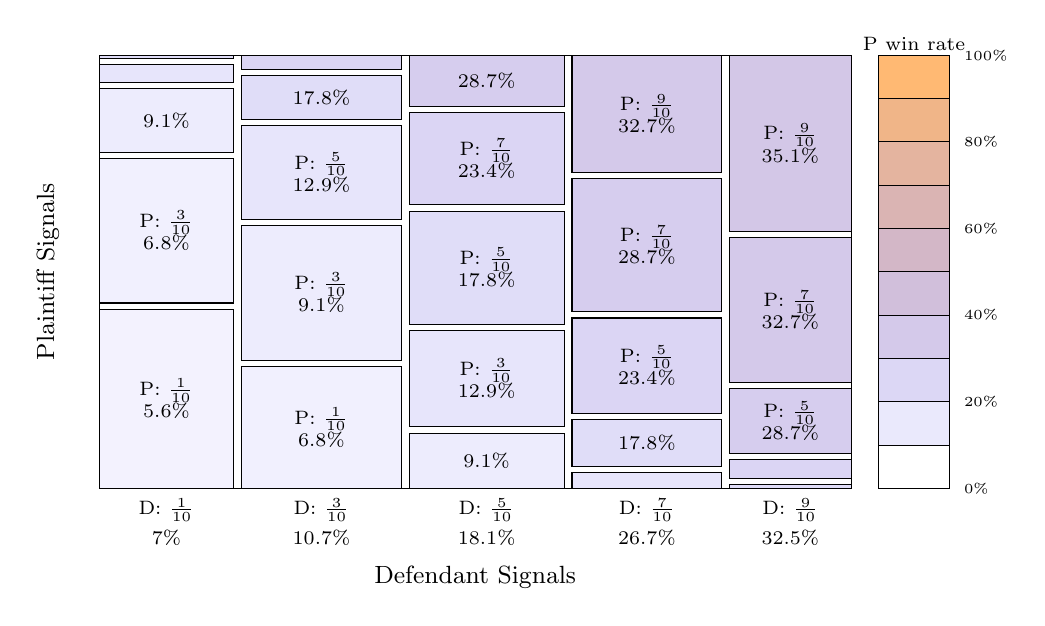
\begin{tikzpicture}
\newcommand{\DFractionOffset}{0.4}
\newcommand{\AxisLabelYAdjust}{-0.235}
\draw[draw=black] (0.6,2) rectangle (10.15,7.5);
\draw[fill=blue!94!orange!6!white!86!white, draw=black] (0.6,2) rectangle (2.3097,4.2744);
\draw (1.4548309132515453, 3.137181222412532) node[font=\scriptsize, text=black, align=center] {P: $\frac{1}{10}$\\ 5.6\%};
\draw[fill=blue!93!orange!7!white!86!white, draw=black] (0.6,4.3544) rectangle (2.3097,6.1894);
\draw (1.4548309132515453, 5.271871996601169) node[font=\scriptsize, text=black, align=center] {P: $\frac{3}{10}$\\ 6.8\%};
\draw[fill=blue!91!orange!9!white!85!white, draw=black] (0.6,6.2694) rectangle (2.3097,7.077);
\draw (1.4548309132515453, 6.673194946537016) node[font=\scriptsize, text=black, align=center] {9.1\%};
\draw[fill=blue!87!orange!13!white!84!white, draw=black] (0.6,7.157) rectangle (2.3097,7.3789);
\draw[fill=blue!82!orange!18!white!82!white, draw=black] (0.6,7.4589) rectangle (2.3097,7.5);
\draw (1.4548309132515453, 1.6) node[anchor=north, font=\scriptsize, text=black] {7\%};
\draw (1.4548309132515453, {1.6 + \DFractionOffset}) node[anchor=north, font=\scriptsize, text=black] {D: $\frac{1}{10}$};
\draw[fill=blue!93!orange!7!white!86!white, draw=black] (2.4097,2) rectangle (4.437,3.5475);
\draw (3.4233256490791786, 2.773743237741831) node[font=\scriptsize, text=black, align=center] {P: $\frac{1}{10}$\\ 6.8\%};
\draw[fill=blue!91!orange!9!white!85!white, draw=black] (2.4097,3.6275) rectangle (4.437,5.3399);
\draw (3.4233256490791786, 4.483712931324461) node[font=\scriptsize, text=black, align=center] {P: $\frac{3}{10}$\\ 9.1\%};
\draw[fill=blue!87!orange!13!white!84!white, draw=black] (2.4097,5.4199) rectangle (4.437,6.6051);
\draw (3.4233256490791786, 6.012518216369952) node[font=\scriptsize, text=black, align=center] {P: $\frac{5}{10}$\\ 12.9\%};
\draw[fill=blue!82!orange!18!white!82!white, draw=black] (2.4097,6.6851) rectangle (4.437,7.2405);
\draw (3.4233256490791786, 6.962796035821291) node[font=\scriptsize, text=black, align=center] {17.8\%};
\draw[fill=blue!77!orange!23!white!80!white, draw=black] (2.4097,7.3205) rectangle (4.437,7.5);
\draw (3.4233256490791786, 1.6) node[anchor=north, font=\scriptsize, text=black] {10.7\%};
\draw (3.4233256490791786, {1.6 + \DFractionOffset}) node[anchor=north, font=\scriptsize, text=black] {D: $\frac{3}{10}$};
\draw[fill=blue!91!orange!9!white!85!white, draw=black] (4.537,2) rectangle (6.5057,2.7013);
\draw (5.5213654895863264, 2.350671054194941) node[font=\scriptsize, text=black, align=center] {9.1\%};
\draw[fill=blue!87!orange!13!white!84!white, draw=black] (4.537,2.7813) rectangle (6.5057,4.0018);
\draw (5.5213654895863264, 3.3915517338252714) node[font=\scriptsize, text=black, align=center] {P: $\frac{3}{10}$\\ 12.9\%};
\draw[fill=blue!82!orange!18!white!82!white, draw=black] (4.537,4.0818) rectangle (6.5057,5.5201);
\draw (5.5213654895863264, 4.800942204540098) node[font=\scriptsize, text=black, align=center] {P: $\frac{5}{10}$\\ 17.8\%};
\draw[fill=blue!77!orange!23!white!80!white, draw=black] (4.537,5.6001) rectangle (6.5057,6.7711);
\draw (5.5213654895863264, 6.185606231059471) node[font=\scriptsize, text=black, align=center] {P: $\frac{7}{10}$\\ 23.4\%};
\draw[fill=blue!71!orange!29!white!79!white, draw=black] (4.537,6.8511) rectangle (6.5057,7.5);
\draw (5.5213654895863264, 7.1755447061497035) node[font=\scriptsize, text=black, align=center] {28.7\%};
\draw (5.5213654895863264, 1.6) node[anchor=north, font=\scriptsize, text=black] {18.1\%};
\draw (5.5213654895863264, {1.6 + \DFractionOffset}) node[anchor=north, font=\scriptsize, text=black] {D: $\frac{5}{10}$};
\draw[fill=blue!87!orange!13!white!84!white, draw=black] (6.6057,2) rectangle (8.5074,2.1994);
\draw[fill=blue!82!orange!18!white!82!white, draw=black] (6.6057,2.2794) rectangle (8.5074,2.8715);
\draw (7.556572810241555, 2.575494980380009) node[font=\scriptsize, text=black, align=center] {17.8\%};
\draw[fill=blue!77!orange!23!white!80!white, draw=black] (6.6057,2.9515) rectangle (8.5074,4.1638);
\draw (7.556572810241555, 3.5576834338267975) node[font=\scriptsize, text=black, align=center] {P: $\frac{5}{10}$\\ 23.4\%};
\draw[fill=blue!71!orange!29!white!79!white, draw=black] (6.6057,4.2438) rectangle (8.5074,5.933);
\draw (7.556572810241555, 5.088393782859181) node[font=\scriptsize, text=black, align=center] {P: $\frac{7}{10}$\\ 28.7\%};
\draw[fill=blue!67!orange!33!white!77!white, draw=black] (6.6057,6.013) rectangle (8.5074,7.5);
\draw (7.556572810241555, 6.756482740786128) node[font=\scriptsize, text=black, align=center] {P: $\frac{9}{10}$\\ 32.7\%};
\draw (7.556572810241555, 1.6) node[anchor=north, font=\scriptsize, text=black] {26.7\%};
\draw (7.556572810241555, {1.6 + \DFractionOffset}) node[anchor=north, font=\scriptsize, text=black] {D: $\frac{7}{10}$};
\draw[fill=blue!82!orange!18!white!82!white, draw=black] (8.6074,2) rectangle (10.15,2.0456);
\draw[fill=blue!77!orange!23!white!80!white, draw=black] (8.6074,2.1256) rectangle (10.15,2.3615);
\draw[fill=blue!71!orange!29!white!79!white, draw=black] (8.6074,2.4415) rectangle (10.15,3.2697);
\draw (9.378702056482862, 2.8556045868982802) node[font=\scriptsize, text=black, align=center] {P: $\frac{5}{10}$\\ 28.7\%};
\draw[fill=blue!67!orange!33!white!77!white, draw=black] (8.6074,3.3497) rectangle (10.15,5.1829);
\draw (9.378702056482862, 4.266277776111093) node[font=\scriptsize, text=black, align=center] {P: $\frac{7}{10}$\\ 32.7\%};
\draw[fill=blue!65!orange!35!white!76!white, draw=black] (8.6074,5.2629) rectangle (10.15,7.5);
\draw (9.378702056482862, 6.381430972274309) node[font=\scriptsize, text=black, align=center] {P: $\frac{9}{10}$\\ 35.1\%};
\draw (9.378702056482862, 1.6) node[anchor=north, font=\scriptsize, text=black] {32.5\%};
\draw (9.378702056482862, {1.6 + \DFractionOffset}) node[anchor=north, font=\scriptsize, text=black] {D: $\frac{9}{10}$};
\node[font=\small, text=black] at (5.375, {1.1 + \AxisLabelYAdjust}) {Defendant Signals};
\node[font=\small, text=black, rotate=90] at (-0.050000000000000044, 4.75) {Plaintiff Signals};
\draw[draw=black] (10.5,2) rectangle (11.4,7.5);
\draw (10.95, 7.65) node[font=\scriptsize, text=black] {P win rate};
\draw[fill=blue!100!orange!0!white!88!white, draw=black] (10.5,2) rectangle (11.4,2.55);
\draw[fill=blue!89!orange!11!white!84!white, draw=black] (10.5,2.55) rectangle (11.4,3.1);
\draw[fill=blue!78!orange!22!white!81!white, draw=black] (10.5,3.1) rectangle (11.4,3.65);
\draw[fill=blue!67!orange!33!white!77!white, draw=black] (10.5,3.65) rectangle (11.4,4.2);
\draw[fill=blue!56!orange!44!white!73!white, draw=black] (10.5,4.2) rectangle (11.4,4.75);
\draw[fill=blue!44!orange!56!white!70!white, draw=black] (10.5,4.75) rectangle (11.4,5.3);
\draw[fill=blue!33!orange!67!white!66!white, draw=black] (10.5,5.3) rectangle (11.4,5.85);
\draw[fill=blue!22!orange!78!white!62!white, draw=black] (10.5,5.85) rectangle (11.4,6.4);
\draw[fill=blue!11!orange!89!white!59!white, draw=black] (10.5,6.4) rectangle (11.4,6.95);
\draw[fill=blue!0!orange!100!white!55!white, draw=black] (10.5,6.95) rectangle (11.4,7.5);
\draw (11.46, 2) node[anchor=west, font=\tiny, text=black] {0\%};
\draw (11.46, 3.1) node[anchor=west, font=\tiny, text=black] {20\%};
\draw (11.46, 4.2) node[anchor=west, font=\tiny, text=black] {40\%};
\draw (11.46, 5.3) node[anchor=west, font=\tiny, text=black] {60\%};
\draw (11.46, 6.4) node[anchor=west, font=\tiny, text=black] {80\%};
\draw (11.46, 7.5) node[anchor=west, font=\tiny, text=black] {100\%};


\end{tikzpicture}
\end{document}